\documentclass[12pt, a4paper]{article}
\title{Beginner's Guide to Competitive Programming With C++}
\author{Mohammad Osoolian}
%\author{Mohammad Osoolian \thanks{Funded by the IUST university.}}
%Links and URLs SETUP
\usepackage{url}
\usepackage{hyperref}
\hypersetup{
    colorlinks=true,
    linkcolor=blue,
    filecolor=magenta,      
    urlcolor=cyan,
    pdftitle={Overleaf Example},
    pdfpagemode=FullScreen,
    }

% C++ code highlighter SETUP
\usepackage{listings}
\usepackage{color}

\definecolor{dkgreen}{rgb}{0,0.6,0}
\definecolor{gray}{rgb}{0.5,0.5,0.5}
\definecolor{mauve}{rgb}{0.58,0,0.82}

\lstset{frame=tb,
  language=c++,
  aboveskip=3mm,
  belowskip=3mm,
  showstringspaces=false,
  columns=flexible,
  basicstyle={\small\ttfamily},
  numbers=none,
  numberstyle=\tiny\color{gray},
  keywordstyle=\color{blue},
  commentstyle=\color{dkgreen},
  stringstyle=\color{mauve},
  breaklines=true,
  breakatwhitespace=true,
  tabsize=3
}

% graphics and images SETUP
\usepackage{float}
\usepackage{graphicx}
\graphicspath{ {./images/} }


\date{February 2023}
\begin{document}
\maketitle
\tableofcontents
\newpage

\section{Why C++?}
There are many different options in programming languages to start competitive programming (CP). However, most of CP competitors choose C++ because of its many benefits. If you still aren't sure if using C++ is the right choice for you, here are some reasons why it might be the best option.
\begin{description}
\item[Faster:] The most important reason is that C++ is much faster than many other languages. In real contest, there is no difference between time limit of various languages. Therefor, those submits with faster languages have more chance of being finished in the specified time limit.
\item[More clear:] C++ is a simple language and it's much closer to machine language. Therefor, in writing C++ code, every thing is just clear for you and no extra operatoin is done behind your code. This is an important adventage that prevents you from making mistakes in calculating time and memory complexity.
\item[Various algorithm tools:] C++ has wide different tools for algorithms that you probably need to use in CP problems. It also has different kinds of data structures that can be very helpful for you.
\item[Widely used:]  C++ is considered to be the best choice for CP problems by 75\% of the programmers across the world. This brings a huge community and great support for you. For example you can use snippets, templates, some data structure implementations and many algorithms implemented in C++.
\end{description}

\section{C++ for competitive programming}
Learning a language for CP problems is actually much easier than learning that language for developing applications. Furthermore, even the rules and conventions of competitive programming differs from programming as a developer. C++ is a powerful language with a lot of tools and libraries and learning all of them might be confusing for you. However, you don't have to learn everything about C++. The only things you need is basic syntax and some useful datatypes and functions and some special conventions for CP that we will talk about later.
\subsection{Basic syntax}
If you're already familiar with any programming language, it will probably be easy for you to learn C++ syntax as well. You only need to learn simple topics, including input, output, variables, conditions, loops and functions. Additionaly, C++ contains a variable type called ''pointer'' that you may have not heard of before. It's a good idea to search about it and get familiar with it. Here are some useful links:
\begin{itemize}
\item \url{https://www.w3schools.com/cpp/cpp_syntax.asp}
\item \url{https://www.tutorialspoint.com/cplusplus/cpp_basic_syntax.htm}
\item \url{https://www.codecademy.com/learn/c-plus-plus-for-programmers/modules/basic-syntax-in-cpp/cheatsheet}
\end{itemize}
Don't try to get too deep into it! You'll learn as much as you need as you go.

\subsection{Important Data types}
\begin{description}
\item[vector:] Just like arrays, vectors use contiguous storage locations for their elements, which means that their elements can also be accessed using indexes, and just as efficiently as in arrays. But unlike arrays, their size can change dynamically, with their storage being handled automatically by the container.

\url{https://www.mygreatlearning.com/blog/vectors-in-c/}
\item[pair:] Pair is used to combine together two values that may be of different data types. Pair provides a way to store two heterogeneous objects as a single unit. It is basically used if we want to store tuples. Pair in C++ behaves similarly to tuple in python. It consists of two elements {first, second}. The first element is referred to as first while the second element is referred to as second. This order must be fixed (first, second).

\url{https://www.scaler.com/topics/cpp/pair-in-cpp/}
\item[queue:] Queues are a type of container adaptors that operate in a first in first out (FIFO) type of arrangement. Elements are inserted at the back (end) and are deleted from the front.

\url{https://www.programiz.com/cpp-programming/queue}
\item[stack:] Stacks are a type of container adaptors with LIFO(Last In First Out) type of working, where a new element is added at one end (top) and an element is removed from that end only

\url{https://www.programiz.com/cpp-programming/stack}
\item[priority\_queue:] A C++ priority queue designed such that the first element of the queue is either the greatest or the smallest of all elements in the queue. We can also change it to the smallest element at the top

\url{https://www.mygreatlearning.com/blog/priority-queue-in-cpp/}
\end{description}

\subsection{Important functions}
\begin{description}
\item[min, max, minmax:] These functions are used to get the minimum, maximum, or both between two or more objects. Additionally, a comparer function can be passed to these functions.

\url{https://www.educative.io/courses/cpp-standard-library-including-cpp-14-and-cpp-17/7nYWrLv9jkQ}

\item[max\_element, min\_element:] max\_element and min\_element return an iterator pointing to the element with the largest or smallest value in the range [first, last). The comparisons can be performed using a pre-defined function.

\url{https://www.geeksforgeeks.org/max_element-in-cpp/}
\item[swap:] This function swaps the values of two variables of any data type.

\url{https://www.geeksforgeeks.org/swap-in-cpp/}
\item[gcd:] C++ builtin function gcd or \_\_gcd in c++14 and before, calculates the gcd of two numbers.

\url{https://www.geeksforgeeks.org/stdgcd-c-inbuilt-function-finding-gcd/}
\item[sort:] This is a very useful functoin in C++ algorithm header that sorts an array or a vector of elements in O(nlogn). It is possible to pass a comparer function to sort elements in a specific order.

\url{https://www.educative.io/answers/what-is-the-stdsort-function-in-cpp}
You can also use a lambda function instead of defining a comparer function. Check this link:

\url{https://stackoverflow.com/questions/5122804/how-to-sort-with-a-lambda}
\item[any\_of, all\_of, none\_of:] These functinos loop over a vector or an array and check if any, all or none of elements have a specific condition. You can pass a boolian function as the condition or write a lambda function in parameters.

\url{https://www.geeksforgeeks.org/any_of-function-in-cpp-stl/}

\url{https://www.geeksforgeeks.org/stdnone_of-in-c/}

\url{https://www.geeksforgeeks.org/stdall_of-in-cpp/}
\item[unique:] Removes all but the first element from every consecutive group of equivalent elements in the range [first,last)

\url{https://www.geeksforgeeks.org/stdunique-in-cpp/}
\item[lower\_bound, upper\_bound:] These functions are used to find bounds of an elements in vectors and arrays and sets. They work in $O(logN)$ for arrays and vectors and can be used instead of writing binary search functions.

\url{https://jimmy-shen.medium.com/lower-bound-and-upper-bound-of-c-2f635619fa97}
\item[\_\_builtin\_popcount:] Counts the number of bits set to 1 of an integer a. This function is specialy used in working with bitmasks.

\url{https://www.geeksforgeeks.org/cpp-__builtin_popcount-function/}
\end{description}

\section{Competitive programming conventions}
Competitive programming has its own rules and conventions. By being aware of these conventions, you can avoid unnecessary details and focus on more important aspects.
\subsection{Problem Conventions}
CP problems have a special form most of the time. They usually have \textbf{Title}, \textbf{Description}, \textbf{Input}, \textbf{Output}, \textbf{Example} and \textbf{Notes}.\footnote{The conventions written in this guide is based on \href{https://codeforces.com/}{codeforces.com}.} Here is a \href{https://codeforces.com/contest/1767/problem/B}{sample problem} on \href{https://codeforces.com/}{Codeforces(CF)} for you to make the explanations below clearer.

\begin{description}
\item[Title:] This part contains the name of the problem, the time limit, and the memory limit. These limitations are really important because it's impossible to answer the question without considering them. However, they usually don't change much. Time limits are usually around 1 or 2 seconds and memory limits are usually around 256 megabytes
\item[Description:] The main explanation of problem is in the Description. You should read this section carefully to understand what exactly the problem is.
\item[Input:] In this section you will find out how inputs of problem are passed to you and how you should read them. There is another important piece of information here which is \textbf{input boundaries}. Input boundaries show you how much the inputs can get bigger. For example it shows you how long the length of input array could be, or how many queries exist in one test case at most. Input boundaries are really important because they can help you determine the order of time complexity of your answer.

\emph{Normal computers can do $3\cdot10^8$ operations in one second}. Therefore, assuming that you have one array as input and boundary of length of array(N) is $1 < N < 10^5$, then your answer has to be at most in $O(NlogN)$. Sometimes you can discover what techniques and data structures to use if you know the suitable time complexity of the answer.

\item[Output:] the Output section tells you how you should print your answers. Sometimes they should be printed in oneline, sometimes in multiple lines, sometimes with spaces between, sometimes with out it, sometimes in lower case, and sometimes in upper case. Make sure you print exactly the same output as the problem wants. Answers are corrected by machine. Therefore, even a little differnece can make your answer incorrect.
\item[Example:] After explaining the problem and the form of input and output, an example is given to you in this part to ensure that you understand the concept of the problem. \emph{Always try your code with the examples before submitting}.
\item[Notes:] Finally, in the last part, there are some explanations for the examples above. If you cannot understand the concept of the problem, read this section carefully and try to figure out the relationship between the input and output in the examples.
\end{description}

\subsection{Code Conventions}
CP problems coding has a different style from other fields of coding. For example, when coding for a web project, the goal is to keep the project up and secure; it needs to be maintained, developed, and get new features. So your code must follow clean code rules to be easy to read and modifiable for other developers.

However, in CP, the only goal of coding is to pass the tests and get the score of problem in the shortest time possible. But that doesn't mean that you shouldn't follow clean code rules. Actually, to achieve this goal and get the highest score, your code must be clean, but in a different way.

That is because some of the clean code rules of big projects take so much time from you, causing you to lose points for latency. To solve this problem, some rules have been changed in a way that takes less time from you while still keeping your code clean and easy to read at the same time.

In conclusion, in CP, coding has different purposes and values compared to other contexts of coding, so don't expect the rules to be exactly the same as the coding rules you have heard before.

In this section, you will learn some conventions in CP coding, with help of this \href{https://codeforces.com/contest/1767/submission/185533520}{code} submitted for this \href{https://codeforces.com/contest/1767/problem/B}{question} in CF.

\begin{figure}[H]
\fbox{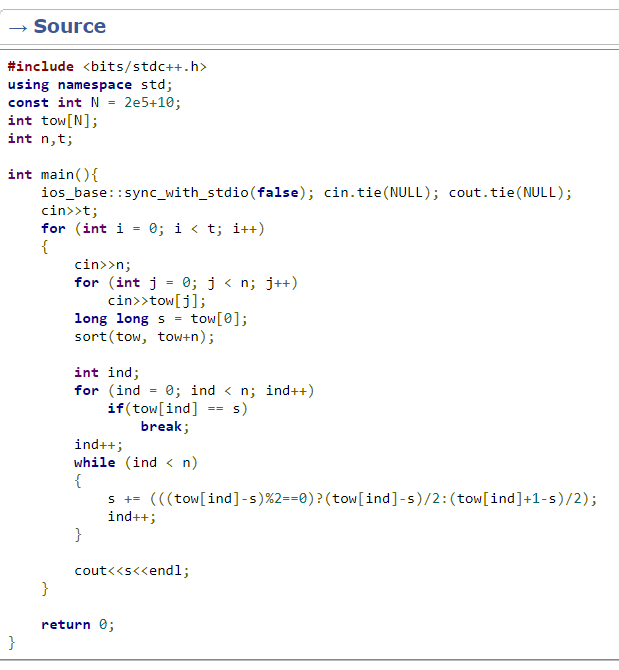
\includegraphics[scale=1]{sample_submit_half}}
\caption{sample submitted code}
\end{figure}

\subsubsection{Headers}
% \begin{description}
%\item[Including headers]:
There are some frequently used standard libraries in CP problems that may not be needed in every problem you solve. However, competitors usually include all of them regardless of whether they are necessary to use or not. The reason for that is because it is just easier and takes less time comparing to include every library just when you need it in the code. There could be also a \lstinline{using namespace std;} after including libraries for convinience and to reduce code.

here are the list of frequent used standard libraries\footnote{\href{https://gist.github.com/kodekracker/e09f9d23573f117a5db0}{source}}:

\begin{lstlisting}
#include <iostream>
#include <string>
#include <vector>
#include <algorithm>
#include <sstream>
#include <queue>
#include <deque>
#include <bitset>
#include <iterator>
#include <list>
#include <stack>
#include <map>
#include <set>
#include <functional>
#include <numeric>
#include <utility>
#include <limits>
#include <time.h>
#include <math.h>
#include <stdio.h>
#include <string.h>
#include <stdlib.h>
#include <assert.h>

using namespace std;
\end{lstlisting}

However, rather than including all these libraries, you can only include \lstinline{<bits/stdc++>} header. It's not a standard library but contains all necessary headers for CP.

\begin{lstlisting}
#include <bits/stdc++>
using namespace std;
\end{lstlisting}

\begin{figure}[H]
\centering
\fbox{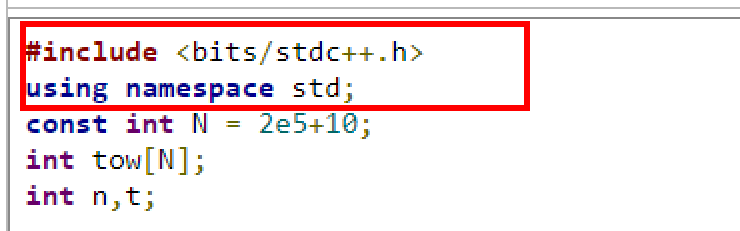
\includegraphics[scale=0.5]{headers}}
\caption{included headers}
\end{figure}

\subsubsection{Constraints}
%\item[Constraints:] 
Constraints come from the input boundaries of the problems. It is a convention among CP competitors to globaly declare \lstinline{const int} variables for baoudaries. Thats because these boundaries are so important in creating arrays and memory needed variables to hold input values. In CP, memory efficiency is not a priority; therefore, the maximum possible number of inputs is considered for creating arrays, and this is where constraints are used.
Look at the example problem and submitted code given at the beginning of this section. 

It is specified in the problem that the number of towers is $2\cdot10^5$ at most. Here $2\cdot10^5$ is a constraint. Therefore, we can write \lstinline{const int N = 2e5;} and use N to initialize arrays we need, or in the better choice we can write \lstinline{const int N = 2e5 + 10}. This addition dosn't change the memory complexity but it could help in preveting from bugs that appear in corner cases.

\begin{itemize}
\item $n\cdot em$ stands for $n\cdot10^m$.
\item This syntax actually returns a \lstinline{float} number, not an \lstinline{int}. For example, in C++, \lstinline{2e3} equals to \lstinline{2000.0} not \lstinline{2000}. Therefore, it is incorrect to write \lstinline{int nums[2e5+10]}. But when you assign this float value to an integer variable like N, C++ casts it to an integer value and after that, you can use the variable to initialize arrays, as in the given example.
\end{itemize}

\begin{figure}[!h]
\centering
\fbox{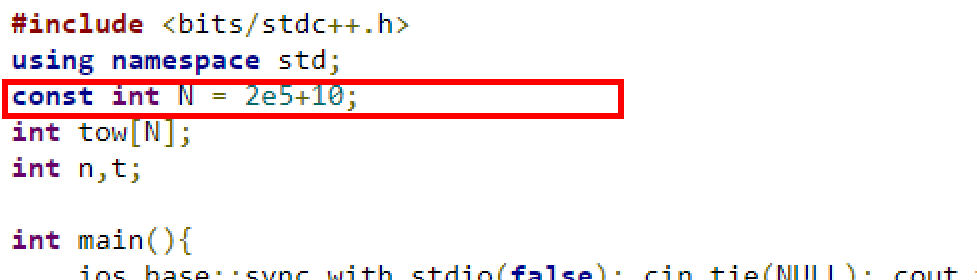
\includegraphics[scale=0.5]{constraints}}
\caption{constraints  of code}
\end{figure}

\subsubsection{Global variables}
%\item[Global variables:] 
Basically, global variables hold everything you read from input, the result of preprocessing on input values, and anything you need in the main function. Number of test cases, length of arrays, the arrays that keep input data, DP arrays, etc, are some examples of frequently used global variables.It is not a good idea to use global variables in large projects; however, in CP contests, the main goal is to write the answer as quickly and easily as possible, and making use of global variables can help a lot. Declaring global variables makes it much easier for you to define functions because you don't have to pass them through function parameters. Instead, you can access them directly.

\begin{figure}[h]
\centering
\fbox{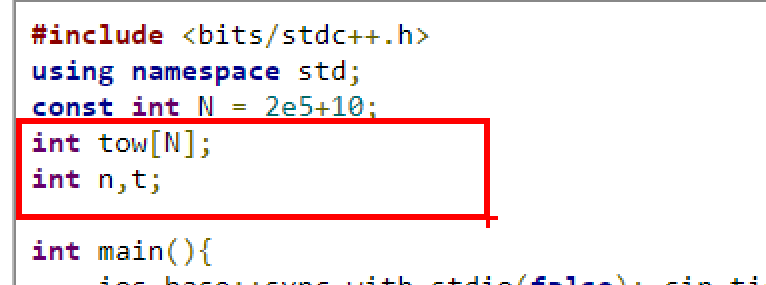
\includegraphics[scale=0.5]{global_variables}}
\caption{global variables}
\end{figure}


\subsubsection{Fast I/O}
%\item[Fast I/O:] 
In some questions, the input size is too large and you lose a lot of time just reading the input, resulting in a time limit error In these cases, you can use \lstinline{scanf} and \lstinline{printf} as a faster method instead of \lstinline{cin} and \lstinline{cout}, or you can add these lines at the beginning of \lstinline{main} function to make \lstinline{cin} and \lstinline{cout} faster.

\begin{lstlisting}
ios_base::sync_with_stdio(false); 
cin.tie(NULL); 
cout.tie(NULL);
\end{lstlisting}
Both ways can solve the problem but the second one is probably easier for you.

\begin{figure}[h]
\fbox{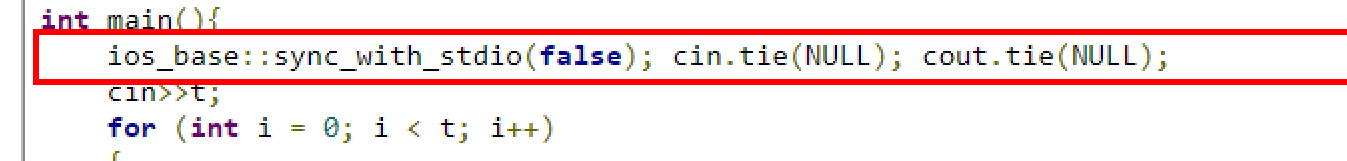
\includegraphics[scale=0.5]{fast_IO2}}
\caption{fast I/O}
\end{figure}

\subsubsection{Typedefs}
%\item[Typedefs:] 
\lstinline{typedef} is a syntax in C++ that allows you to define abbreviations for variable types. Using this syntax, you can code faster and make it shorter and easier to read. Here are some famous typedefs used by many competitors:
\begin{lstlisting}
typedef long long LL;
typedef pair<int, int> pii;
typedef pair<LL, LL> pll;
typedef pair<string, string> pss;
typedef vector<int> vi;
typedef vector<vi> vvi;
typedef vector<pii> vii;
typedef vector<LL> vl;
typedef vector<vl> vvl;
\end{lstlisting}

\subsubsection{Macros}
%\item[Macros:] 
Macros are the \lstinline{#define} statements in C++ and they are another technique of shortening code in CP. Macros are useful in many cased but it's not a good idea to use them too much. In the past, \lstinline{#define} statements were used instead of \lstinline{typedef}, but most of the macros have faster and safer alternatives now. Here is some useful macros:
\begin{lstlisting}
#define PI 3.1415926535897932384626
#define mp make_pair
#define fi first
#define se second
#define DBG(vari) cerr<<#vari<<" = "<<(vari)<<endl;
#define pb push_back
\end{lstlisting}

\subsubsection{Templates}
%\item[Templates:] 
After becoming familiar with all these conventions, you may like some of them and even have your own macros. Now, instead of typing macros every time, you can create a collection of them and make a snippet in your editor that copies and pastes this collection. This collection is called a \textbf{template} in CP. This is my template:

\begin{lstlisting}
#include <bits/stdc++.h>
using namespace std;

#define mp make_pair
#define fi first
#define se second
#define DBG(vari) cerr<<#vari<<" = "<<(vari)<<endl;
#define pb push_back
typedef long long LL;
typedef pair<int, int> pii;
typedef pair<LL, LL> pll;

 
int main(){
    ios_base::sync_with_stdio(false); cin.tie(NULL); cout.tie(NULL);

    return 0;
}
\end{lstlisting}

You can also find more templates on the internet or make your own template and customize it as you like.
%\end{description}

\section{Practice makes perfect}
Now that you are familiar with the rules of Competitive Programming, the only thing left to do is practice. Keep trying and work hard, and you will be able to solve more complex problems in less time. Don't give up easily on difficult problems and try not to look at the answers. Instead, take a break, come back later with fresh ideas.These websites are great for practicing. There are thousands of problems in various levels and topics. There are also exciting contests that you can attend and challenge your self.
\begin{itemize}
\item \href{https://codeforces.com/}{Codeforces}
\item \href{https://www.topcoder.com/}{TopCoder}
\item \href{https://www.codechef.com/}{CodeChef}
\item \href{https://www.hackerrank.com/}{HackerRank}
\end{itemize}



\end{document}